\subsection{Pretraining Ablation Study}

To evaluate the effect of transfer learning, we conduct an ablation study comparing pretrained initialization and random initialization under different optimization settings.

Three experiments are considered:

\begin{enumerate}
    \item The final pretrained baseline configuration selected from hyperparameter search.
    
    \item Random initialization with the same hyperparameters as the pretrained baseline. In this setting, only the pretrained ImageNet initialization is removed, while all optimization settings remain unchanged. This serves as the most controlled ablation experiment.
    
    \item Random initialization with a larger backbone learning rate and longer training schedule. Specifically, the backbone learning rate is increased from $10^{-5}$ to $10^{-3}$, matching the classifier learning rate, and the number of training epochs is increased from 30 to 50.
\end{enumerate}

\begin{figure}[H]
    \centering
    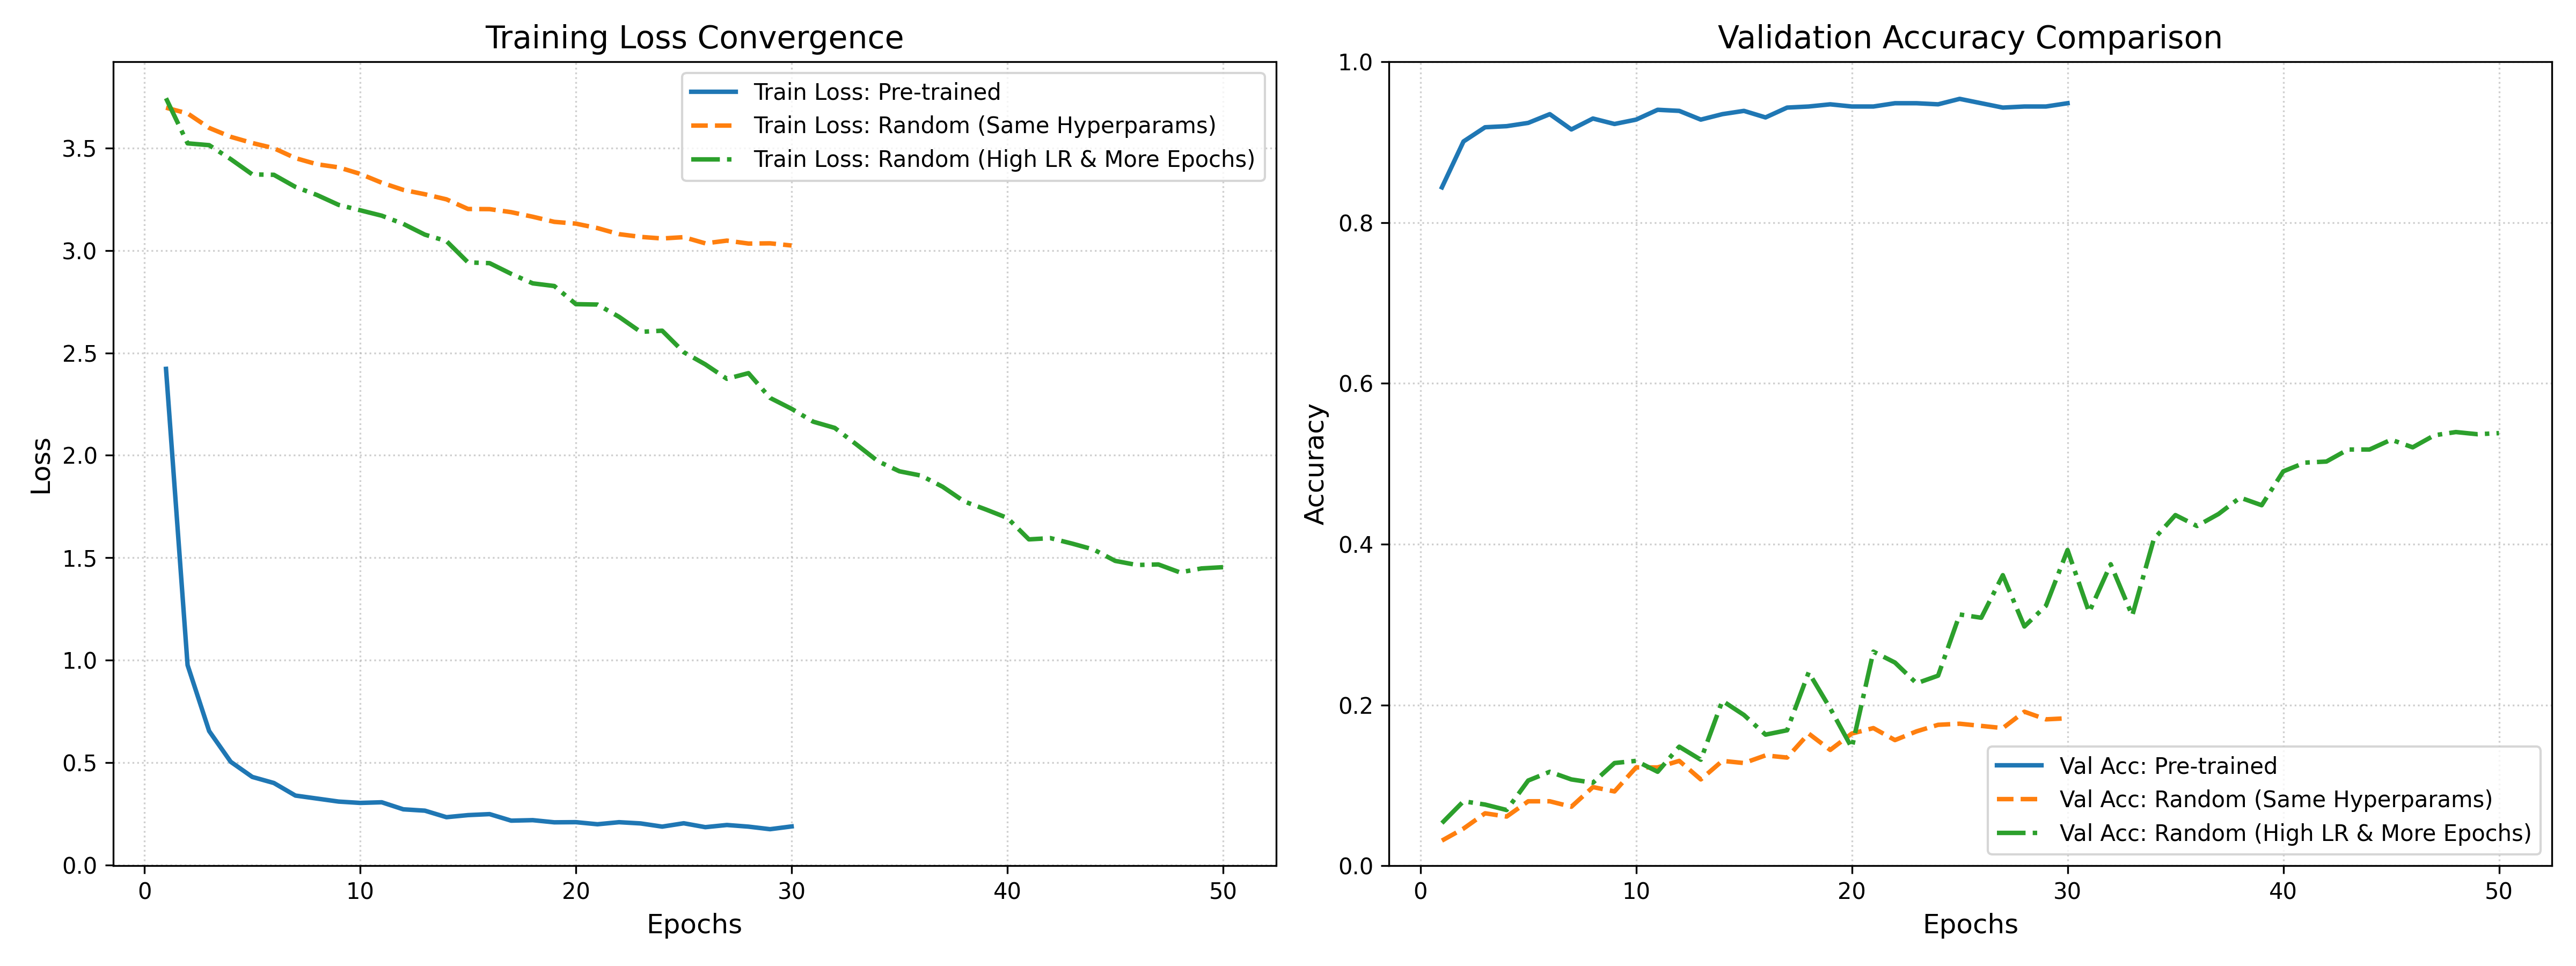
\includegraphics[width=0.85\textwidth]{figures/task1/ablation_results.png}
    \caption{Comparison between pretrained initialization and random initialization. Left: training loss curves. Right: validation accuracy curves.}
    \label{fig:ablation_results}
\end{figure}

The final validation accuracies are summarized below:

\begin{table}[H]
\centering
\caption{Validation accuracy in the pretraining ablation study.}
\label{tab:pretraining_ablation}
\begin{tabular}{l c}
\toprule
Configuration & Validation Accuracy \\
\midrule
Pretrained initialization & 0.9538 \\
Random initialization (same hyperparameters) & 0.1916 \\
Random initialization + larger LR + longer training & 0.5394 \\
\bottomrule
\end{tabular}
\end{table}

The results demonstrate the importance of pretrained initialization for transfer learning on the Oxford-IIIT Pet dataset. Under the same optimization settings, the randomly initialized model fails to converge effectively and achieves extremely poor validation accuracy.

The training curves in Figure~\ref{fig:ablation_results} further show that pretrained models converge significantly faster and achieve consistently lower training loss throughout training.

Comparing the two randomly initialized settings, increasing the backbone learning rate substantially accelerates optimization and improves validation accuracy. This observation suggests that the small backbone learning rate used for pretrained fine-tuning is unsuitable for randomly initialized models, whose backbone parameters require much larger updates during early training. Nevertheless, even after increasing the learning rate and extending training to 50 epochs, the randomly initialized model still performs substantially worse than the pretrained counterpart.
